En este capitulo describimos en detalles los pasos para realizar la transformación, utilizaremos el modelo ya presentado e introduciremos un modelo PowerDEVS con componentes vectoriales con el fin de ilustrar la transformación de estos componentes.

\section{Modelos DEVS}

        \subsection{Archivos PDS}
        PowerDEVS trabaja principalmente con dos archivos, .PDM y .PDS.
        Los archivos PDM es utilizado por el editor de modelos, pues contiene información estructural, así como información de posición de los modelos dentro del 
        editor, sus parámetros, lo cual indica nombre, tipo y valor, descripción de los modelos, la cantidad de puertos de cada modelo y las conexiones
        entre los modelos, los detalles de como esas conexiones son visualizadas por lineas y los detalles del recorrido de esas lineas. 
        Todos estos elementos son utilizados en primera medida con el editor de modelos, pero tambien son utilizados para generar el archivo PDS el cual es el 
        genera el código de la simulación.
        El archivo PDS contiene información estructural del modelo necesaria para realizar la simulación, en el listado \ref{lst:pdsstruc} se pueden ver un 
        esbozo de su estructura.
        
\begin{listing}[H]
\begin{minted}{text}
Root-Coordinator
 {
  Simulator
   {
    Path = vector\qss_sum_vec.h
    Parameters = "1","-1","1","0","0","0","0","0",3.000000e+00,"N"
   }
   ...
    Coordinator
     {
      ...
     }
   ...     
  Simulator
   {
        ...
   }
  EIC
   {
   }
  EOC
   {
   }
  IC
   {
        ...
   }
 }
\end{minted}
\caption{Estructura de un archivo PDS.}
\label{lst:pdsstruc}
\end{listing}

        Se puede observar un elemento \texttt{Root-Coordinator} el cual contiene (marcado entre llaves) una lista de \texttt{Simulator} que representan 
	los modelos atómicos y/o \texttt{Coordinator} que representan los modelos acoplados y tres listas de 
        conexiones \texttt{EIC}, \texttt{EOC} y \texttt{IC}, conexiones de entrada externa (External Input Connections), 
        conexiones de salida externa (external output connections) y conexiones internas (Internal Connections).

	Las lista de conexiones internas (IC) es una lista de par de pares de números naturales, de la forma $(a,b);(c,d)$.
	Donde el primer par se refiere al origen de la conexión (puerto $b$ de salida) del modelo $a$ y el segundo al fin de la conexion (puerto $d$ de entrada) 
	del modelo $c$, ambos modelos se refiere a la lista de modelos (atómicos o acoplados) del actual modelo.
	Es decir el par $(0,0);(1,0)$ indica que el puerto $0$ del segundo modelo (posición 1) es de entrada  y esta conectado al puerto $0$ del primer modelo.

	Tanto EIC y EOC siguen el mismo patron excepto que replazan el modelo de los puertos de salida y extrada respectivamente por $0$. Es decir el elemento 
	$(6,0);(0,1)$ en EOC indica que el puerto $0$ del modelo $6$ (septima posición)  se encuentra conectado con el puerto $1$ de salida del modelo 
	acoplado, y un par $(0,0);(2,1)$ en EIC indica que el primer puerto (puerto $0$) se encuentra conectado con el modelo 2 (tercera posición) en su puerto $1$.

        Los modelos acoplados dado que también son modelos DEVS, replican la estructura listado \ref{lst:pdsstruc}.

        Para poder leer esta estructura se cuenta con la librería de PowerDEVS\footnote{http://sourceforge.net/p/powerdevs/code/HEAD/tree/} la cual nos permite acceder
        a la estructura desde C++. 

\section{Modelos Atómicos}
	
	Internamente los modelos atómicos son identificados por el parámetro \texttt{Path} en el archivo PDS, para realizar la tradución de este modelo se utiliza 
	un modelo Modelica el cual debe seguir la siguiente especificación:

\begin{itemize}
	\item El código debe ser Modelica ($\mu$-modelica) valido y estar ubicado en el mismo directorio (y nombre del archivo) del código C que el modelo atómico 
	PowerDEVS, con el mismo nombre que el archivo .h, pero con extensión .mo, es decir un modelo con \texttt{vector\textbackslash qss\_sum\_vec.h} utilizara un modelo 
	\texttt{vector/qss\_sum\_vec.h} \footnote{El nombre de los archivos se replaza \quotes{\textbackslash} por \quotes{/} para permitir algunos modelos 
	cuyos \texttt{Path} contiene ese separadores de directorios}
	\item Los parámetros del modelo DEVS deben ser pasado en el parámetro $p$
	\item Los valores de entrada del modelo son asociados a la variable $u$
	\item Los valores de salida del modelos son asociados a la variable $y$
\end{itemize}

	Por ejemplo el código del integrador, originalmente ubicado en el archivo qss\_integrator.h de PowerDEVS, se ubica en el archivo qss\_integrator.mo mostrado en el listado 
	\ref{lst:qssintegrator.mo} ambos dentro del directorio qss.

\begin{listing}[H]
\begin{minted}{modelica}
class QSSIntegrator
        parameter Real p[4]={0,0,0,0,0,0,0,0};
  parameter Real x0 = p[4];
  Real u[1];
  Real y[1](start = {x0});
equation
  der(y[1]) = u[1];
end QSSIntegrator;
\end{minted}
\caption{Modelo qss\_integrator.mo}
\label{lst:qssintegrator.mo}
\end{listing}

	El modelo Lotka Volterra cuenta con dos integradores (con los mismo parámetros) representados en el listado \ref{lst:qssint.pds}, en este se puede ver el \texttt{Path} y \texttt{Parameters}
	que componen todos los modelos atómicos.

\begin{listing}[H]
\begin{minted}{text}
  ...
  Simulator
   {
    Path = qss/qss_integrator.h
    Parameters = "QSS3","1e-6","1e-3","0.5"
   }
   ...
\end{minted}
\label{lst:qssint.pds}
\caption{Extracto del modelo Lotka Volterra, modelo atómico de un integrator.}
\end{listing}

	Luego de remplazar los parámetros en la variable \texttt{p}, se prefijan todas las variables por el nombre del modelo y su posición en este caso con el prefijo 
	\quotes{\texttt{QSSIntegrator\_1\_}}

\begin{listing}[H]
\begin{minted}{modelica}
class QSSIntegrator
  parameter Real QSSIntegrator_1_p[4]={0,1e-6, 1e-3, 0.5};
  parameter Real QSSIntegrator_1_x0 = p[4];
  Real QSSIntegrator_1_u[1];
  Real QSSIntegrator_1_y[1](start = {QSSIntegrator_1_x0});
equation
  der(QSSIntegrator_1_y[1]) = QSSIntegrator_1_u[1];
end QSSIntegrator;
\end{minted}
\caption{Transformación parcial de un modelo atómico de un integrator en el modelo de ejemplo Lotka Volterra.}
\end{listing}



	Los parámetros son remplazadas en el modelo, evaluados en Scilab\footnote{Para realizar la evaluación en Scilab se utiliza el mismo mecanismo que 
	provee (y utiliza) PowerDEVS.}, lo que los transforma en float, los cuales son presentados como reales (Real) en el código.

	Los modelos no encontrados son ignorados en la traducción y se reportan en el registro (log) de la conversión.

\section{Modelos Acoplados Planos}

Llamamos \emph{Modelos Acoplados Planos} a los Modelos Acoplados que solo contienen \emph{Modelos Atómicos}. Estos modelos son convertidos en modelos Modelica de la siguiente forma:
Para el $i$-esimo modelo atómico del modelo acoplado
\begin{itemize}
        \item Se incluye el código Modelica del $i$-esimo modelo atómico
        \item Se remplazan los parámetros $p$ por los del $i$-esimo modelo atómico.
        \item Se reescriben todas las variables (excepto la variable $time$) construido con $i$ y el nombre del modelo (en Modelica).
\end{itemize}

Luego cada conexión entre Modelos Atómicos es replicada en el código de Modelica resultante. Los modelos Atómicos cuyo entrada (o salida) son escalares son conectados con un ecuación del tipo $u = y$ mientras que los modelos vectoriales son conectados con la misma ecuación, solo que dentro de un $for$.

Veamos como se realiza la transformación paso a paso con un ejemplo de un integrador.

\begin{figure}[!htbp]
\begin{center}
  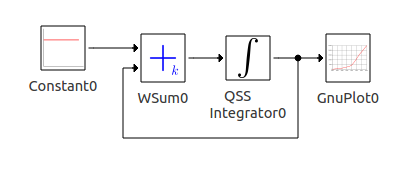
\includegraphics[scale=0.5]{integrator-devs}
  \caption{DEVS Ejemplo de Integrador}
  \end{center}
   \label{fig:integrator}
\end{figure}

Este modelo incluye los siguientes modelos atómicos:
\begin{itemize}
        \item Constante: Constant0
\begin{minted}{modelica}        
class Constant
  parameter Real k = 1;
  Real y[1];
equation
  y[1] = k;
end Constant;
\end{minted}

        \item Sumador: WSum0
\begin{minted}{modelica}        
class WSum
  parameter Real p[9]={0,0,0,0,0,0,0,0};
  parameter Integer n= integer(p[9]);
  parameter Real w[n] = p[1:n];
  Real u[n];
  Real y[1];
equation
  y[1]=u*w;
end WSum;
\end{minted}

        \item Integrador: QSSIntegrator0
\begin{minted}{modelica}        
class QSSIntegrator
  parameter Real p[4]={0,0,0,0,0,0,0,0};
  parameter Real x0 = p[4];
  Real u[1];
  Real y[1](start = {x0});
equation
  der(y[1]) = u[1];
end QSSIntegrator;
\end{minted}

        \item Gnu Plot : GNUPlot0, el cual no va a ser convertido debido a que no tiene un modelo equivalente en modelica.
\end{itemize}

El integrador es el primero en la lista de atómicos dentro del PowerDEVS, por lo que es el primero en procesarse y por lo tanto obtiene el prefijo $<nombre modelo>\_0\_$ para sus variables, también remplazamos los parámetros provenientes de la simulación de PowerDEVS:

\begin{minted}{modelica}        
class QSSIntegrator
  parameter Real QSSIntegrator_0_p[4]={0,1e-06,0.001,0};
  parameter Real QSSIntegrator_0_x0 = 0;
  Real QSSIntegrator_0_u[1];
  Real QSSIntegrator_0_y[1](start = {QSSIntegrator_0_x0});
equation
  der(y[1]) = QSSIntegrator_0_u[1];
end QSSIntegrator;
\end{minted}

\begin{minted}{modelica}
class WSum
  parameter Real WSum_1_p[9]={1,(-1),0,0,0,0,0,0,2};
  parameter Integer WSum_1_n= integer(2);
  parameter Real WSum_1_w[WSum_1_n] = p[1:WSum_1_n];
  Real WSum_1_u[WSum_1_n];
  Real WSum_1_y[1];
equation
  WSum_1_y[1]=WSum_1_u*WSum_1_w;
end WSum;
\end{minted}

\begin{minted}{modelica}        
class Constant
  parameter Real Constant_2_k = 1;
  Real Constant_2_y[1];
equation
  Constant_2_y[1] = Constant_2_k;
end Constant;   
\end{minted}

En este punto podemos juntar las declaraciones y ecuaciones dentro de un nuevo modelo, el cual llamaremos con el nombre del modelo a convertir.

\begin{minted}{modelica}        
class Integrador
  parameter Real QSSIntegrator_0_p[4]={0,1e-06,0.001,0};
  parameter Real QSSIntegrator_0_x0 = 0;
  Real QSSIntegrator_0_u[1];
  Real QSSIntegrator_0_y[1](start = {QSSIntegrator_0_x0});
  parameter Real WSum_1_p[9]={1,(-1),0,0,0,0,0,0,2};
  parameter Integer WSum_1_n= integer(2);
  parameter Real WSum_1_w[WSum_1_n] = p[1:WSum_1_n];
  Real WSum_1_u[WSum_1_n];
  Real WSum_1_y[1];
equation
  der(y[1]) = QSSIntegrator_0_u[1];
  WSum_1_y[1]=WSum_1_u*WSum_1_w;
  Constant_2_y[1] = Constant_2_k;
end QSSIntegrator;
\end{minted}

Luego de agregar las equaciones correspondientes a las interconecciones de los modelos atómicos, obtenemos el siguiente modelo
        
\begin{minted}{modelica}
model Integrador
  parameter Real QSSIntegrator_0_p[4] = {0,1e-06,0.001,0};
  parameter Real QSSIntegrator_0_x0 = 0;
  Real QSSIntegrator_0_u[1];
  Real QSSIntegrator_0_y[1](start = {0});
  parameter Real WSum_1_p[9] = {1,(-1),0,0,0,0,0,0,2};
  parameter Integer WSum_1_n = integer(2);
  parameter Real WSum_1_w[WSum_1_n] = WSum_1_p[1:WSum_1_n];
  Real WSum_1_u[WSum_1_n];
  Real WSum_1_y[1];
  parameter Real Constant_2_k = 1;
  Real Constant_2_y[1];
  equation
    der(QSSIntegrator_0_y[1]) = QSSIntegrator_0_u[1];
    WSum_1_y[1] = WSum_1_u*WSum_1_w;
    Constant_2_y[1] = 1;
    QSSIntegrator_0_u[1] = WSum_1_y[1];
    WSum_1_u[2] = QSSIntegrator_0_y[1];
    WSum_1_u[1] = Constant_2_y[1];
end Integrador;
\end{minted}

\section{Modelos Acoplados Jerárquicos}
En la sección anterior mostramos como son convertidos modelos acoplados compuestos por modelos atómicos, para convertir un modelo acoplado jerárquico, es decir con más modelos acoplados internos, vamos a generar un modelo acoplado plano, equivalente al modelo jerárquico inicial.

Para realizar el aplanado, se recorre recursivamente los modelos acoplados:

\begin{itemize}
\item por cada modelo acoplado si solo tiene modelos atómicos, es remplazado por los modelos atómicos internos, los cuales se encuentran conectados sin modificaciones excepto por las conexiones externas, las cuales son reasignadas de forma de mantener las conexiones.
\item si el modelo acoplado contiene otros modelos acoplados entonces aplanamos ese modelo recursivamente.
\end{itemize} 

De esta forma obtenemos un modelo con solo modelos atómicos el cual podemos convertir con el procedimiento anterior.

A modo de ejemplo se muestran, el esquema del integrador de la sección anterior con un modelo acoplado en \ref{fig:acomplado} y luego el mismo modelo en \ref{fig:aplanado}, aplanado, el cual puede ser convertido pues ya no presenta jerarquias.

\begin{figure}[H]
\centering
 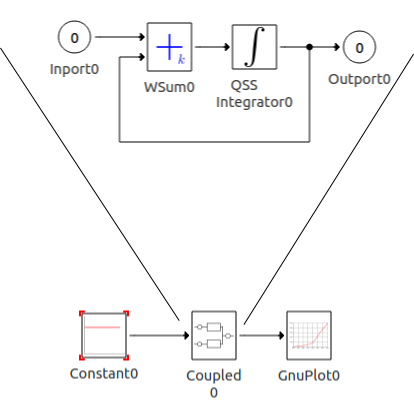
\includegraphics[width=0.5\linewidth]{integrator-sample}
 \caption{Representación de un modelo simple de integrador acoplado}
 \label{fig:acomplado}
\end{figure}


\begin{figure}[H]
\centering
 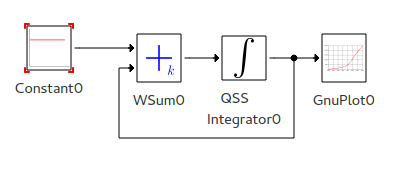
\includegraphics[width=0.5\linewidth]{integrator-expanded}
 \caption{Representación del modelo de integrador aplanado }
 \label{fig:aplanado}
\end{figure}



\section{Modelos Vectoriales}
Los modelos vectoriales difieren levemente de los atómicos no vectoriales. Estos modelos pueden tener tanto la entrada como la salida de sus conectores de forma vectorial, por lo que los modelos vectoriales deben indicarlos con la anotación de Modelica $PD2MO$, por ejemplo:
\begin{itemize}
\item $annotation(PD2MO = {Scalar, Vector});$ cuando la entrada es escalar, es decir no vectorial y la salida vectorial
\item $annotation(PD2MO = {Vector, Scalar});$ cuando la entrada es vectorial y la salida vectorial
\item $annotation(PD2MO = {Vector, Vector});$ cuando ambos, la entrada y salida son vectoriales.
\item $annotation(PD2MO = {Scalar, Scalar});$ cuando ambas entrada y salida son escalares, este es el caso por omisión y no es necesario declararlo.
\end{itemize}

Además las variables de entradas $u$ y salidas $y$ vectoriales deben ser definidas como vectores en Modelica. A modo de ejemplo se muestra a continuación el archivo vector/qss\_integrator\_vec.mo. Este modelo atómico representa $N$ integradores y es la version vectorial del integrador atómico mostrado antes.

\begin{minted}{modelica}
class VecInt
  parameter Real p[5] = {0, 10, 0, 0, 10};
  constant Integer N = p[5];
  parameter Real x0 = p[4];
  Real u[N, 1];
  Real y[N, 1];
initial algorithm
  for i in 1:N loop
    y[i, 1] := x0;
  end for;
equation
  for i in 1:N loop
    der(y[i, 1]) = u[i, 1];
  end for;
  annotation(PD2MO = {Vector, Vector});
end VecInt;
\end{minted}


\section{Equivalencia semántica de la conversión}
Hay tres situaciones que debemos considera al momento de verificar la equivalencia semántica
\begin{itemize}
\item Modelos Atómicos : Los modelos atómicos son convertidos por el usuario, los que se han propuesto en el código mantienen una conservación de la semántica que no es estricta y se trató manualmente. 
\item Modelos Acoplado - Plano : Como fue descripto en la sección Modelos Acoplados Planos, los modelos son conectados por una ecuación en caso de ser un modelo escalar, o por un conjunto de ecuaciones (expresadas en una sentencia $for$). En este caso esta conversión (conexión por igualdad) no mantiene la semántica, pues la semántica de una conexión (o grupo de conexiones en el caso vectorial) es diferente de la semántica de un ecuación (o grupos de ecuaciones).

\item Modelo Jerárquico : En este caso si podemos probar la equivalencia semántica, entre el modelo original, es decir un modelo acoplado que incluye más modelos acoplados, con un modelo \quotes{aplanado} (solo con modelos atómicos). Esto se debe a que el formalismo DEVS es cerrado bajo el acoplamiento \cite{Zeigler:2000:TMS:580780} y \cite{zeigler1984multifacetted}, lo que permite remplazar un modelos acoplado por equivalentes atómicos, conectados apropiadamente.
\end{itemize}
